\chapter{Resultados y validación experimental}
\label{cap:resultados}

\section{Diseño de la evaluación}

Para valorar el comportamiento del sistema no basta con indicar que genera una nota. Lo relevante es comprobar cómo responde ante casos representativos, si distingue respuestas correctas, parciales e incorrectas, y hasta qué punto su calificación se aproxima a la de un corrector humano. Por ese motivo la validación se ha planteado en varios niveles, de menor a mayor exigencia: un análisis cualitativo de casos, una batería determinista con notas esperadas, pruebas de robustez ante respuestas tramposas, un banco de exámenes que cubre varios niveles educativos, una medida de concordancia mediante correlación de Spearman frente a notas de referencia y, finalmente, una validación contra notas de profesores humanos reales sobre un conjunto de datos externo.

Conviene una advertencia metodológica que se mantiene a lo largo del capítulo. En las pruebas propias, las notas humanas con las que se compara el sistema son \emph{de referencia}: las ha asignado el autor según rúbrica, emulando el criterio de un profesor del nivel correspondiente. No proceden de un tribunal real. Sirven para medir la concordancia con un criterio explícito, no la exactitud absoluta. La única excepción es la validación externa, donde las notas sí son de correctores humanos reales.

\section{Análisis cualitativo de tres casos}

Como punto de partida se analizan tres respuestas de comportamiento claramente distinto sobre la misma pregunta de biología celular, con los conceptos clave \emph{mitocondria}, \emph{energía}, \emph{ATP} y \emph{respiración celular}. La tabla~\ref{tab:casos} las resume. La primera cubre por completo el contenido; la segunda expresa una comprensión parcial; la tercera utiliza un término del dominio, pero lo relaciona de forma incorrecta.

\begin{table}[ht]
\centering
\caption{Evaluación semántica sobre tres respuestas representativas.}
\label{tab:casos}
\small
\begin{tabularx}{\textwidth}{>{\raggedright\arraybackslash}p{0.16\textwidth} >{\raggedright\arraybackslash}X >{\raggedright\arraybackslash}p{0.10\textwidth}}
\toprule
Tipo & Texto y conceptos & Nota \\
\midrule
Correcta & ``La mitocondria es un orgánulo que produce energía en forma de ATP mediante la respiración celular.'' Detecta todos los conceptos. & 8--10 \\
Parcial & ``La mitocondria produce energía para la célula.'' Detecta mitocondria y energía; respiración celular parcial; ATP ausente. & $\sim 6$ \\
Incorrecta & ``La mitocondria es el núcleo de la célula.'' El término aparece, pero no sostiene una relación válida. & $<4$ \\
\bottomrule
\end{tabularx}
\end{table}

El interés de estos casos es que la diferencia entre ellos no depende de una sola señal, sino de la interacción entre varias decisiones de diseño. La respuesta correcta se beneficia de una cobertura conceptual completa y una similitud alta. La parcial conserva una nota media porque aporta parte del contenido nuclear, pero no encuentra ATP y solo recibe evidencia parcial de \emph{respiración celular}. La incorrecta queda por debajo de 4 porque la mera presencia del término ``mitocondria'' no activa evidencia válida cuando la relación semántica es errónea. Este comportamiento evita uno de los fallos clásicos de la corrección automática: premiar respuestas incorrectas que reutilizan el vocabulario del tema.

\section{Batería de validación determinista}

Para poder detectar regresiones de forma sistemática, se construyó una batería de validación (\texttt{validate.py}) con 40 casos repartidos en dos asignaturas, Biología e Informática, agrupados por tema. Cada caso fija una respuesta y una banda de nota esperada, y se considera conforme si la nota del sistema cae dentro de la banda. La batería incluye respuestas completas, parciales, triviales y adversarias, además de cinco casos específicos de negación y polaridad.

En su estado actual, la batería arroja un comportamiento conforme del 100\,\%: 39 casos pasan dentro de su banda y un único caso falla de forma esperada (está marcado como tal, pues comprueba precisamente una limitación conocida). Esta batería actúa como red de seguridad: cualquier cambio en el grader se contrasta contra ella antes de darse por bueno, lo que permitió, por ejemplo, detectar de inmediato un falso positivo introducido por el análisis de polaridad, descrito más adelante. El conjunto de pruebas del proyecto, ejecutado de forma automática, supera las doscientas comprobaciones unitarias y de integración.

\section{Evaluación del reconocimiento óptico}

Como el sistema parte de imágenes, conviene cuantificar el eslabón del OCR en lugar de darlo por bueno. Para ello se renderizaron respuestas reales del banco con una tipografía estándar y se sometieron a degradaciones típicas de un escaneo o una fotografía —desenfoque, ruido, rotación y baja resolución—, midiendo el error de lectura por carácter (CER) y por palabra (WER), y, sobre todo, la diferencia de nota entre corregir el texto original y corregir el texto leído por OCR. Es importante delimitar el alcance: esta prueba evalúa texto \textbf{impreso}, no manuscrito; el reconocimiento de escritura a mano es un problema distinto y más difícil, reconocido como límite del trabajo. Por tanto, estas cifras son un límite optimista respecto a un examen manuscrito real.

\begin{table}[ht]
\centering
\caption{Robustez del OCR de texto impreso ante degradaciones de imagen (14 respuestas, idioma español).}
\label{tab:ocr}
\small
\begin{tabular}{lccc}
\toprule
Condición & CER & WER & $|\Delta\text{nota}|$ media \\
\midrule
Limpio & 0\,\% & 0\,\% & 0{,}00 \\
Baja resolución & 0{,}8\,\% & 4{,}3\,\% & 0{,}00 \\
Rotación (4\textdegree) & 25{,}2\,\% & 31{,}5\,\% & 0{,}28 \\
Desenfoque & 6{,}8\,\% & 22{,}7\,\% & 1{,}58 \\
Ruido fuerte & 100\,\% & 100\,\% & 9{,}62 \\
\bottomrule
\end{tabular}
\end{table}

La tabla~\ref{tab:ocr} muestra un comportamiento revelador. Con imagen limpia o de baja resolución, el OCR de texto impreso es prácticamente perfecto y la nota no cambia. Lo más interesante es la rotación: produce un 25\,\% de error de caracteres pero solo $0{,}28$ puntos de diferencia en la nota, porque lo que importa para la corrección es que sobrevivan los conceptos clave, no cada letra; el pipeline absorbe el error gracias a la detección parcial y la tolerancia. El ruido fuerte, en cambio, es el punto de ruptura: destruye la lectura y, con ella, la nota. La conclusión es que, para texto impreso en condiciones razonables, el OCR no es el cuello de botella del sistema, y que el módulo semántico aporta una robustez adicional frente a errores moderados de lectura.

\section{Robustez ante respuestas tramposas}

Un corrector serio debe resistir dos trampas que un comparador de conceptos ingenuo no detecta: negar los términos correctos y atribuirlos a otro objeto. La tabla~\ref{tab:robustez} muestra el comportamiento del sistema sobre la pregunta de la mitocondria.

\begin{table}[ht]
\centering
\caption{Comportamiento ante respuestas adversarias (nota sobre 10).}
\label{tab:robustez}
\small
\begin{tabularx}{\textwidth}{>{\raggedright\arraybackslash}X c c}
\toprule
Respuesta del alumno & Sin polaridad & Con el sistema actual \\
\midrule
``La mitocondria \emph{no} produce ATP ni realiza la respiración celular.'' & 9{,}84 & \textbf{0{,}3} \\
``Esos procesos son cosa del cloroplasto, \emph{no} de la mitocondria.'' & 9{,}84 & 9{,}9 + \emph{revisar} \\
``La mitocondria no \emph{solo} produce ATP, sino que respira\dots'' & --- & 9{,}85 \\
\bottomrule
\end{tabularx}
\end{table}

La negación explícita la resuelve el módulo determinista de polaridad: la respuesta falsa cae de 9{,}84 a 0{,}3, mientras que la construcción enfática ``no solo\dots\ sino'' no se penaliza. La atribución errónea, en cambio, escapa a lo determinista —los términos se afirman, solo que referidos al objeto equivocado—; ahí interviene el verificador, que mantiene la nota del grader pero marca el caso para revisión, clasificando los tres conceptos como atribución errónea. La combinación de ambos mecanismos cubre las dos trampas sin volverse indulgente ni injusto con las respuestas correctas que usan negaciones legítimas.

\section{El efecto de los sinónimos: banco de exámenes por nivel}

La prueba más amplia es un banco de exámenes conceptuales (\texttt{exam\_bank.py}) que cubre cinco niveles educativos: Primaria, ESO, Bachillerato, Universidad (Ingeniería Informática) y Máster. Reúne 33 preguntas de un abanico de asignaturas y, para cada una, tres respuestas de alumno —de nivel notable, aprobado y suspenso— con su nota de referencia, lo que suma 99 respuestas calificadas. El sistema corrige cada respuesta y se compara su nota con la de referencia mediante la correlación de Spearman, que mide la concordancia de \emph{orden}, y el error absoluto medio (MAE), que mide la distancia en la escala de 0 a 10.

Este banco fue, además, la prueba que reveló con más claridad la limitación de las paráfrasis descrita en la sección~\ref{sec:sinonimos}: el sistema infravaloraba respuestas correctas expresadas con palabras propias. La tabla~\ref{tab:banco} compara la concordancia antes y después de incorporar los sinónimos por concepto.

\begin{table}[ht]
\centering
\caption{Concordancia con la nota de referencia en el banco por niveles, antes y después de los sinónimos por concepto.}
\label{tab:banco}
\small
\begin{tabular}{lcccc}
\toprule
 & \multicolumn{2}{c}{Sin sinónimos} & \multicolumn{2}{c}{Con sinónimos} \\
\cmidrule(lr){2-3}\cmidrule(lr){4-5}
Métrica (global, $N=99$) & Spearman & MAE & Spearman & MAE \\
\midrule
Resultado & $+0{,}872$ & $1{,}44$ & $\mathbf{+0{,}931}$ & $\mathbf{0{,}96}$ \\
\bottomrule
\end{tabular}
\end{table}

La incorporación de los sinónimos elevó la correlación global de Spearman de $0{,}872$ a $0{,}931$, redujo el error medio de $1{,}44$ a $0{,}96$ puntos sobre 10 y rebajó la proporción de discrepancias importantes (desviaciones de 2{,}5 puntos o más respecto a la referencia) del 24\,\% al 9\,\%. La tabla~\ref{tab:niveles} muestra el detalle por nivel con la versión final del sistema.

\begin{table}[ht]
\centering
\caption{Concordancia por nivel educativo (versión con sinónimos).}
\label{tab:niveles}
\small
\begin{tabular}{lccc}
\toprule
Nivel & $N$ & Spearman & MAE \\
\midrule
Primaria & 15 & $+0{,}95$ & $0{,}72$ \\
ESO & 21 & $+0{,}91$ & $0{,}89$ \\
Bachillerato & 21 & $+0{,}94$ & $1{,}19$ \\
Universidad & 24 & $+0{,}94$ & $1{,}07$ \\
Máster & 18 & $+0{,}92$ & $0{,}81$ \\
\bottomrule
\end{tabular}
\end{table}

\begin{figure}[ht]
\centering
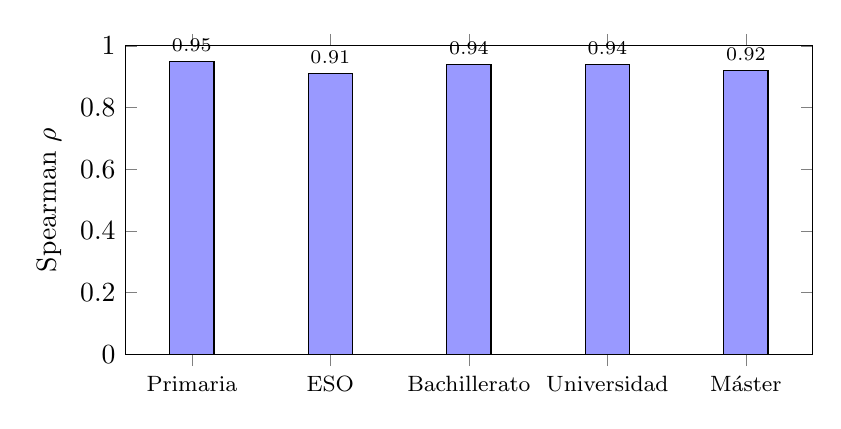
\begin{tikzpicture}
\begin{axis}[
  ybar, bar width=16pt, width=0.85\textwidth, height=5.5cm,
  ymin=0, ymax=1, ylabel={Spearman $\rho$},
  symbolic x coords={Primaria,ESO,Bachillerato,Universidad,Máster},
  xtick=data, x tick label style={font=\footnotesize},
  nodes near coords, nodes near coords style={font=\scriptsize},
  enlarge x limits=0.12]
\addplot[fill=blue!40] coordinates {(Primaria,0.95)(ESO,0.91)(Bachillerato,0.94)(Universidad,0.94)(Máster,0.92)};
\end{axis}
\end{tikzpicture}
\caption{Correlación de Spearman por nivel educativo (versión con sinónimos).}
\label{fig:spearman-nivel}
\end{figure}

El sistema ordena las respuestas como un corrector de referencia en todos los niveles, de Primaria a Máster, sin que la correlación caiga en ningún tramo por debajo de $0{,}91$ (figura~\ref{fig:spearman-nivel}). El banco fue también útil para depurar el sistema: destapó un falso positivo del detector de negación, en el que el ``no'' de ``no metales'' marcaba como negados los conceptos posteriores de una respuesta de Química y hundía un notable de 10 a 6; el error se corrigió añadiendo ``no metales'' a las excepciones léxicas. De las nueve discrepancias que quedan, dos son sobrevaloraciones por presencia de términos sin coherencia —las que marca el verificador— y siete son infravaloraciones de respuestas genuinamente incompletas, donde el alumno solo nombra parte de la rúbrica; que una respuesta a medias obtenga menos nota que una completa es el comportamiento correcto. La tabla~\ref{tab:discrep} las clasifica.

\begin{table}[ht]
\centering
\caption{Clasificación de las nueve discrepancias restantes en el banco por niveles.}
\label{tab:discrep}
\small
\begin{tabularx}{\textwidth}{>{\raggedright\arraybackslash}p{0.28\textwidth} c >{\raggedright\arraybackslash}X}
\toprule
Asignatura / nivel & Tipo & Causa \\
\midrule
Lengua (ESO) & Sobrevalora & Términos correctos en una afirmación falsa \\
Biología (Bach.) & Sobrevalora & ``Consume oxígeno'': proceso invertido \\
Estructuras de Datos (Univ.) & Infravalora & Respuesta incompleta (solo el concepto central) \\
Sistemas Operativos (Univ.) & Infravalora & Respuesta incompleta \\
Filosofía (Bach.) $\times 2$ & Infravalora & No reproduce el término técnico exacto \\
Programación (Univ.) & Infravalora & Respuesta incompleta \\
Machine Learning (Máster) & Infravalora & Respuesta incompleta \\
Matemáticas (Bach.) & Infravalora & Falta un concepto de la rúbrica \\
\bottomrule
\end{tabularx}
\end{table}

Las dos sobrevaloraciones son, precisamente, los casos para los que existe el verificador; las infravaloraciones reflejan respuestas a las que un profesor concede el beneficio de la duda y que el sistema, más literal, califica algo por debajo. Ninguna de las dos categorías es un fallo de funcionamiento: delimitan el margen de error esperable.

\section{Correlación de Spearman sobre un conjunto de referencia}

Para disponer de una medida de concordancia más exigente que las bandas de la batería determinista, se construyó un conjunto de 30 respuestas con nota de referencia repartida por toda la escala, sobre seis preguntas de Biología e Informática (\texttt{gold\_dataset.py}). Sobre este conjunto, el sistema obtiene una correlación de Spearman de $0{,}87$, una correlación de Pearson de $0{,}91$ y un error medio de $1{,}2$ puntos sobre 10. El propio experimento expone, además, las costuras del enfoque: una pregunta de fotosíntesis baja su correlación porque una respuesta incorrecta que ``consume oxígeno'' es sobrevalorada por presencia de términos, un caso que el verificador detectaría. La figura~\ref{fig:scatter} representa la nota del sistema frente a la de referencia para las 30 respuestas; la diagonal marca el acuerdo perfecto. La mayoría de los puntos se sitúan cerca de ella, y las desviaciones se concentran en la zona media, coherentes con la tendencia del sistema a ser algo más severo con las respuestas intermedias.

\begin{figure}[ht]
\centering
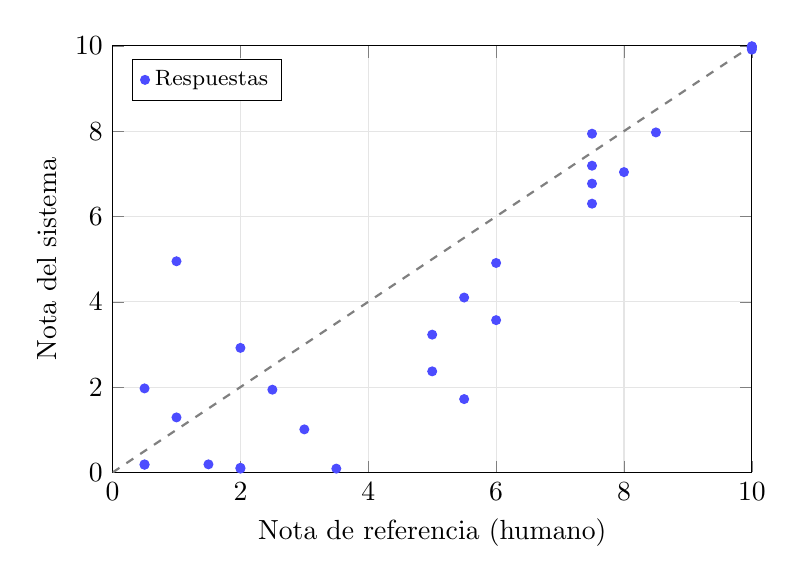
\begin{tikzpicture}
\begin{axis}[
  width=0.8\textwidth, height=7cm,
  xlabel={Nota de referencia (humano)}, ylabel={Nota del sistema},
  xmin=0,xmax=10,ymin=0,ymax=10, grid=both, grid style={gray!20},
  legend pos=north west, legend style={font=\footnotesize}]
\addplot[domain=0:10, dashed, gray, thick, forget plot] {x};
\addplot[only marks, mark=*, mark size=1.6pt, blue!70] coordinates {
 (10,9.99)(7.5,6.3)(5.5,4.1)(2.5,1.94)(0.5,1.97)
 (10,9.97)(8.5,7.97)(6,4.91)(3,1.01)(1,4.95)
 (10,9.96)(7.5,7.19)(5,3.23)(2,0.11)(0.5,0.19)
 (10,9.97)(7.5,7.94)(5,2.37)(2,0.09)(0.5,0.18)
 (10,9.91)(7.5,6.77)(5.5,1.72)(1.5,0.19)(2,2.92)
 (10,9.98)(8,7.04)(6,3.57)(3.5,0.09)(1,1.29)};
\legend{Respuestas}
\end{axis}
\end{tikzpicture}
\caption{Nota del sistema frente a la nota de referencia sobre el conjunto de 30 respuestas. La diagonal discontinua indica el acuerdo perfecto.}
\label{fig:scatter}
\end{figure}

Estas métricas se calculan con una implementación propia de los coeficientes (\texttt{metrics.py}), sin dependencias pesadas, lo que mantiene la coherencia con el carácter interpretable del resto del sistema.

\section{Validación con datos reales: el conjunto de Mohler}

Hasta este punto, todas las notas humanas eran de referencia. La prueba definitiva es contrastar el sistema con notas de profesores humanos reales. Para ello se utilizó el conjunto de \textcite{mohler2011}: 87 preguntas de un curso universitario de informática, en inglés, con unas 2.400 respuestas de alumnos calificadas por dos correctores humanos. El sistema corrige cada respuesta —derivando los conceptos de forma automática a partir de la respuesta de referencia— y se mide su concordancia con la nota humana.

Es importante interpretar este resultado como un \emph{suelo}, no como el mejor caso. El conjunto está en inglés, donde las funciones de negación y sinónimos, diseñadas para el español, no actúan, de modo que solo se prueba el motor base. Además, la rúbrica se deriva automáticamente y es más pobre que una construida por un profesor. La tabla~\ref{tab:mohler} recoge los resultados.

\begin{table}[ht]
\centering
\caption{Concordancia con notas humanas reales (conjunto de Mohler, $N \approx 2400$).}
\label{tab:mohler}
\small
\begin{tabular}{lc}
\toprule
Métrica & Valor \\
\midrule
Spearman global & $+0{,}54$ \\
Pearson & $+0{,}48$ \\
MAE & $4{,}33$ / 10 \\
MAE tras corregir el sesgo de escala & $\mathbf{1{,}63}$ / 10 \\
\bottomrule
\end{tabular}
\end{table}

El dato más informativo no es el error bruto, sino su naturaleza. La media de las notas humanas es $8{,}38$ y la del sistema $4{,}15$: un desfase de más de cuatro puntos. Los correctores de Mohler son muy generosos —el 80\,\% de sus notas son iguales o superiores a 7—, mientras que el sistema es estricto. Al restar ese desfase constante, el error medio cae de $4{,}33$ a $1{,}63$. En otras palabras, el sistema \emph{ordena} las respuestas de forma parecida a los humanos, pero en una escala más severa. El error es sobre todo de escala, no de criterio.

\section{El techo humano: el acuerdo entre dos correctores}

La cifra anterior puede leerse como decepcionante solo si se compara con un ideal de correlación 1. Pero ese ideal no existe ni siquiera entre humanos. El conjunto de Mohler proporciona, además del promedio, las notas de \emph{los dos correctores por separado}, lo que permite la comparación más directa posible: medir cuánto concuerdan los dos profesores entre sí. Esa concordancia humano-humano es el \emph{techo} realista al que puede aspirar cualquier sistema.

Sobre las respuestas con alineamiento verificado entre respuesta y notas (1.868 respuestas), los dos correctores humanos concuerdan con una correlación de Spearman de \textbf{0,60}. El sistema alcanza \textbf{0,55} con el promedio humano. La tabla~\ref{tab:techo} lo resume, con intervalos de confianza al 95\,\% obtenidos por \emph{bootstrap}.

\begin{table}[ht]
\centering
\caption{Concordancia humano-humano (techo) frente a la del sistema, conjunto de Mohler.}
\label{tab:techo}
\small
\begin{tabularx}{\textwidth}{>{\raggedright\arraybackslash}X c c}
\toprule
Comparación & Spearman (IC 95\,\%) & MAE \\
\midrule
Humano 1 vs. Humano 2 (\textbf{techo}) & $+0{,}60$ $[0{,}57,\,0{,}64]$ & $1{,}42$ \\
Sistema vs. promedio humano & $+0{,}55$ $[0{,}52,\,0{,}58]$ & $4{,}39$ \\
Sistema vs. Humano 1 & $+0{,}50$ $[0{,}47,\,0{,}54]$ & $4{,}16$ \\
Sistema vs. Humano 2 & $+0{,}49$ $[0{,}45,\,0{,}52]$ & $4{,}81$ \\
\bottomrule
\end{tabularx}
\end{table}

La figura~\ref{fig:techo} representa estas cifras con sus intervalos de confianza, junto a la línea que marca el techo humano. Se aprecia visualmente que las barras del sistema no quedan lejos de ese techo.

\begin{figure}[ht]
\centering
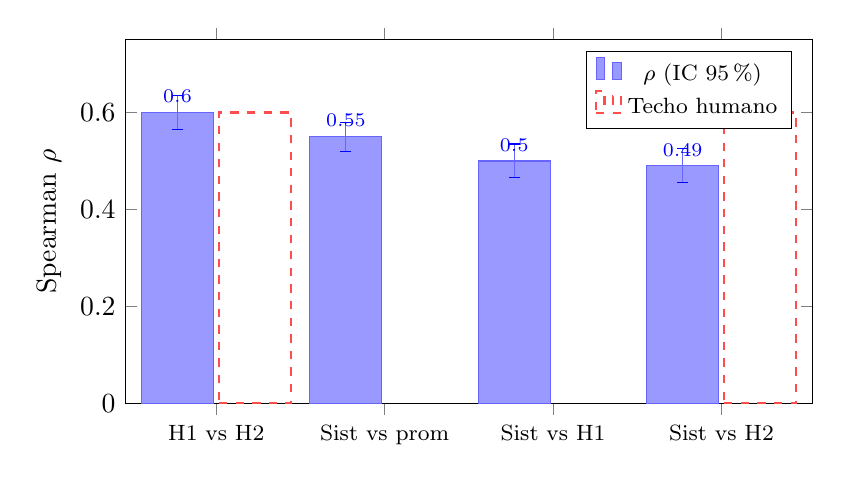
\begin{tikzpicture}
\begin{axis}[
  ybar, bar width=26pt, width=0.85\textwidth, height=6.2cm,
  ymin=0, ymax=0.75, ylabel={Spearman $\rho$},
  symbolic x coords={H1 vs H2, Sist vs prom, Sist vs H1, Sist vs H2},
  xtick=data, x tick label style={font=\footnotesize},
  enlarge x limits=0.18, legend pos=north east, legend style={font=\footnotesize}]
\addplot+[fill=blue!40, draw=blue!60,
         nodes near coords, nodes near coords style={font=\scriptsize},
         error bars/.cd, y dir=both, y explicit]
  coordinates {
    (H1 vs H2,0.60) +- (0,0.035)
    (Sist vs prom,0.55) +- (0,0.03)
    (Sist vs H1,0.50) +- (0,0.035)
    (Sist vs H2,0.49) +- (0,0.035)};
\addplot[dashed, red!70, thick, mark=none] coordinates {(H1 vs H2,0.60) (Sist vs H2,0.60)};
\legend{$\rho$ (IC 95\,\%), Techo humano}
\end{axis}
\end{tikzpicture}
\caption{Acuerdo humano-humano (techo) frente al del sistema sobre el conjunto de Mohler, con intervalos de confianza al 95\,\%. La línea discontinua marca el techo humano ($\rho=0{,}60$).}
\label{fig:techo}
\end{figure}

La lectura cambia por completo. El sistema no concuerda con el promedio humano un poco peor que un humano: concuerda a $0{,}55$ cuando el techo humano es $0{,}60$, es decir, alcanza en torno al \textbf{90\,\% del acuerdo que dos profesores tienen entre sí}, y lo hace en su peor escenario (inglés, rúbrica derivada automáticamente, sin sinónimos). Visto contra ese techo, el resultado deja de ser una cifra pobre y pasa a ser notable. Este es, probablemente, el resultado más importante del trabajo, porque sustituye una comparación con un ideal imposible por una comparación con la realidad: la corrección humana tampoco es perfectamente consistente.

\section{Recalibración sobre datos reales}

El hallazgo anterior justifica la capa de calibración de la sección~\ref{sec:calibracion}. Para comprobar que el desfase se corrige sin circularidad —entrenando y midiendo en datos distintos—, se entrenó el calibrador con el 70\,\% del conjunto de Mohler y se evaluó sobre el 30\,\% restante, no visto durante el ajuste. La tabla~\ref{tab:calibracion} muestra el resultado en ese conjunto de prueba.

\begin{table}[ht]
\centering
\caption{Efecto de la calibración sobre el 30\,\% de Mohler no usado en el ajuste.}
\label{tab:calibracion}
\small
\begin{tabular}{lccc}
\toprule
 & MAE & Pearson & Spearman \\
\midrule
Sin calibrar & $4{,}18$ & $+0{,}47$ & $+0{,}53$ \\
Calibración lineal & $\mathbf{1{,}42}$ & $+0{,}48$ & $+0{,}53$ \\
Calibración isotónica & $1{,}46$ & $+0{,}45$ & $+0{,}53$ \\
\bottomrule
\end{tabular}
\end{table}

El error medio sobre datos no vistos cae de $4{,}18$ a $1{,}42$, lo que demuestra que el desfase era sistemático y se corrige con muy pocas notas del profesor. La correlación de Spearman no cambia, como era de esperar de un mapeo monótono: la calibración no inventa orden, solo ajusta la escala. Ahora bien, conviene no perder de vista un matiz importante. El calibrador lineal ajustado fue, aproximadamente, $\mathrm{nota} = 0{,}34 \cdot \mathrm{cruda} + 7{,}0$, lo que lleva una respuesta cruda de 0 a un 7. Esto no es un defecto del método, sino su consecuencia lógica: la calibración reproduce la generosidad de los correctores de Mohler, incluida su escasa discriminación. La lección es clara: la calibración corrige el desajuste de escala, pero es tan exigente como las notas que la alimentan, y por eso conviene combinarla con rúbricas y sinónimos curados, que sí discriminan.

\section{Enrutado por tipo de pregunta}

Las pruebas anteriores se centran en preguntas conceptuales, que son el ámbito del corrector semántico. Para comprobar el comportamiento sobre un examen heterogéneo se preparó una prueba con preguntas de estilo EvAU de ocho asignaturas, mezclando definiciones, cálculo numérico y redacción. Al pasar \emph{todas} por el corrector semántico, el sistema funcionaba bien en las asignaturas conceptuales (Historia, Filosofía, Química, Economía, Biología) pero fallaba de forma sistemática en cálculo (Matemáticas) y en redacción (Lengua, Lengua extranjera), donde premiaba las palabras clave aunque el resultado fuese incorrecto o la expresión deficiente.

Al activar el enrutado por tipo —corrector semántico para lo conceptual, corrector numérico por equivalencia para el cálculo y juez con rúbrica para la redacción—, las respuestas que antes quedaban mal calificadas pasaron a situarse en la banda que asignaría un profesor. La tabla~\ref{tab:router} resume el cambio: el corrector numérico distingue una conclusión errónea ($x=3$) de la correcta ($x=-3$) aunque ambas citen el símbolo, y el juez de redacción hunde un texto gramaticalmente pobre aunque contenga todo el vocabulario esperado.

\begin{table}[ht]
\centering
\caption{Efecto del enrutado por tipo de pregunta sobre un examen heterogéneo.}
\label{tab:router}
\small
\begin{tabularx}{\textwidth}{>{\raggedright\arraybackslash}p{0.22\textwidth} >{\raggedright\arraybackslash}X c c}
\toprule
Asignatura & Corrector adecuado & Solo semántico & Híbrido \\
\midrule
Historia, Filosofía, Química, Economía, Biología & Semántico & Correcto & Correcto \\
Matemáticas (cálculo) & Numérico (SymPy) & Incorrecto & Correcto \\
Lengua, Lengua extranjera & Juez con rúbrica & Incorrecto & Correcto \\
\bottomrule
\end{tabularx}
\end{table}

La lectura es que el corrector determinista no debe aplicarse indiscriminadamente: su valor está en lo conceptual, y reconocer esa frontera —derivando el resto a un componente específico— es parte del diseño del sistema.

\section{Comparación con una línea base de palabras clave}

Para situar el valor de las mejoras incorporadas conviene compararlas con la alternativa más simple: una corrección por presencia de palabras clave, sin polaridad, sin sinónimos y sin similitud global. Esa línea base, equivalente a comprobar si los términos de la rúbrica aparecen en la respuesta, falla precisamente en los casos que distinguen a un buen corrector de uno ingenuo.

Para cuantificarlo se compararon, sobre el mismo banco, tres correctores: el de solo palabras clave, uno de similitud TF-IDF entre la respuesta y la respuesta ideal (una línea base de similitud más fuerte que la bolsa de palabras, pero que ignora la rúbrica) y el sistema completo. La tabla~\ref{tab:baselines} recoge el resultado, con intervalos de confianza por \emph{bootstrap}.

\begin{table}[ht]
\centering
\caption{Líneas base frente al sistema completo sobre el banco por niveles ($N=99$).}
\label{tab:baselines}
\small
\begin{tabular}{lcc}
\toprule
Método & Spearman (IC 95\,\%) & MAE \\
\midrule
Solo palabras clave & $+0{,}86$ $[0{,}78,\,0{,}92]$ & $1{,}64$ \\
TF-IDF coseno & $+0{,}84$ $[0{,}76,\,0{,}89]$ & $2{,}19$ \\
\textbf{Sistema completo} & $\mathbf{+0{,}93}$ $[0{,}89,\,0{,}95]$ & $\mathbf{0{,}96}$ \\
\bottomrule
\end{tabular}
\end{table}

El sistema supera a ambas líneas base, y la diferencia es mayor en el error medio (0,96 frente a 1,64 y 2,19) que en el orden. Conviene matizar: sobre respuestas conceptuales \emph{limpias} como las del banco, la línea base de palabras clave no es mala ($0{,}86$). Su fragilidad aflora en los casos que el banco no recoge y que sí están en la batería de robustez: en la tabla~\ref{tab:robustez} se vio que una línea base de este tipo otorga un 9{,}84 a una respuesta que niega todo el contenido, mientras que el análisis de polaridad la reduce a 0{,}3. La similitud TF-IDF, por su parte, al ignorar la rúbrica no penaliza lo erróneo ni distingue qué concepto importa. La conclusión es que las mejoras no son adornos: corrigen los errores que harían inservible una corrección simple en un examen real, y lo hacen además mejorando la concordancia agregada.

\section{Reproducibilidad de los resultados}

Una preocupación legítima en cualquier sistema que incorpore un modelo de lenguaje es la reproducibilidad: si las cifras cambian de una ejecución a otra, dejan de ser comparables. En este trabajo, las pruebas que sustentan las tablas anteriores son deterministas, porque el núcleo de corrección lo es: la misma respuesta produce siempre la misma nota. Las funciones que sí dependen de un modelo de lenguaje se invocan con temperatura cero para minimizar su variabilidad, y no intervienen en las métricas de concordancia del corrector, que se calculan únicamente con el grader determinista.

Además, todos los experimentos descritos son reproducibles a partir de los datos incluidos en el proyecto: la batería de validación, el banco de exámenes y los conjuntos de referencia están versionados junto al código, y la validación externa descarga su conjunto de datos de una fuente pública. La separación entre datos y lógica, y la implementación propia de las métricas, hacen que cualquier persona pueda volver a obtener las mismas cifras, lo que es coherente con el énfasis del trabajo en la interpretabilidad y la transparencia de los resultados.

\section{Coste y rendimiento}

Un aspecto a menudo ignorado en la evaluación de un corrector es su coste de ejecución. El núcleo determinista de este sistema realiza, por respuesta, operaciones de texto de complejidad muy baja: normalización, búsqueda de conceptos y un cálculo de similitud sobre vectores de frecuencias. En la práctica, esto significa que la corrección de una respuesta es prácticamente instantánea y que la batería completa de 40 casos, o las 99 respuestas del banco por niveles, se procesan en una fracción de segundo en un equipo personal corriente. El conjunto completo de más de doscientas pruebas automáticas se ejecuta en torno a un segundo.

Este coste contrasta con el de una solución que dependiera de un modelo de lenguaje para cada calificación, donde cada respuesta implicaría una llamada de red, una latencia apreciable y un consumo de recursos varios órdenes de magnitud mayor. Reservar el modelo de lenguaje para funciones opcionales —generación de rúbricas, verificación y juez de redacción— mantiene el coste del flujo principal en niveles despreciables, lo que tiene implicaciones prácticas (la herramienta puede usarse sin coste por uso) y de sostenibilidad. En un escenario de corrección masiva, esta diferencia de coste no es un detalle, sino un factor que condiciona la viabilidad del sistema.

\section{Discusión}

La tabla~\ref{tab:resumen} consolida en un único lugar las medidas de concordancia obtenidas en los distintos escenarios de validación, lo que facilita una lectura comparada.

\begin{table}[ht]
\centering
\caption{Resumen de la validación de concordancia en los distintos escenarios.}
\label{tab:resumen}
\small
\begin{tabularx}{\textwidth}{>{\raggedright\arraybackslash}X c c c}
\toprule
Escenario & $N$ & Spearman & MAE \\
\midrule
Conjunto de referencia (gold) & 30 & $+0{,}87$ & $1{,}2$ \\
Banco por niveles (sin sinónimos) & 99 & $+0{,}87$ & $1{,}44$ \\
Banco por niveles (con sinónimos) & 99 & $\mathbf{+0{,}93}$ & $\mathbf{0{,}96}$ \\
Datos reales (Mohler, sin calibrar) & 1868 & $+0{,}55$ & $4{,}39$ \\
Datos reales (Mohler, calibrado, test) & 733 & $+0{,}53$ & $1{,}42$ \\
\textit{Techo humano-humano (Mohler)} & 1868 & \textit{$+0{,}60$} & \textit{$1{,}42$} \\
\bottomrule
\end{tabularx}
\end{table}

La última fila es la referencia que da sentido al resto: el techo humano-humano. Frente a él, el $0{,}55$ del sistema sobre datos reales no es un suspenso, sino aproximadamente el 90\,\% del acuerdo entre dos profesores.

El conjunto de resultados dibuja un sistema con un comportamiento bien delimitado. Sobre preguntas conceptuales con rúbrica curada y sinónimos —su escenario de diseño— concuerda con la nota de referencia con una correlación de Spearman en torno a $0{,}93$ y un error medio inferior a un punto, de forma consistente en cinco niveles educativos. Resiste las dos trampas clásicas de la corrección por palabras clave gracias a la polaridad determinista y al verificador. Y cuando se enfrenta a datos reales en su peor escenario —otro idioma, sin rúbrica curada— mantiene una concordancia de orden moderada y un error que es casi todo de escala, recuperable con la capa de calibración.

Esa caracterización es, en sí misma, un resultado. La diferencia entre el $0{,}93$ del banco propio y el $0{,}54$ de Mohler no es una contradicción, sino una medida de cuánto dependen el rendimiento de la calidad de la rúbrica y de las funciones específicas del idioma. Antes que presumir de una corrección ``perfecta'', el sistema cuantifica con números cuándo es fiable y cuándo necesita la intervención del profesor, ya sea curando la rúbrica, declarando sinónimos o aportando unas pocas notas para calibrar. Para un sistema pensado como apoyo a la docencia, y no como sustituto del criterio humano, ese reconocimiento de los límites es preferible a una cifra alta sin contexto.
